%!TEX root=../GaugeCNNTheory.tex


\section{Spherical coordinate independent CNNs}
\label{sec:instantiations_spherical}

\begin{figure}
    \centering
    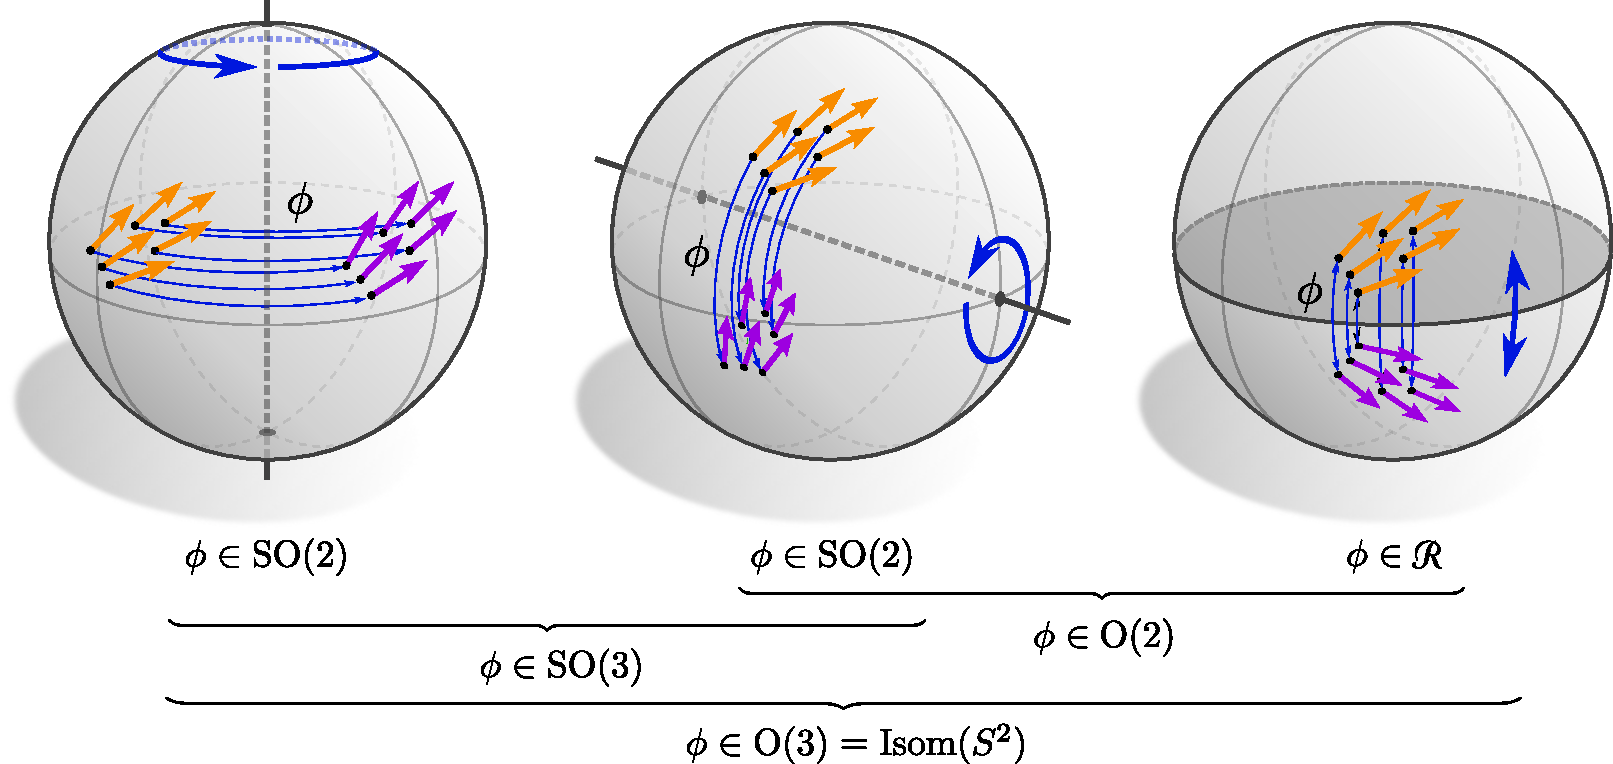
\includegraphics[width=1.\textwidth]{figures/isometry_sphere.pdf}
    \caption{\small
        Visualization of the 2-sphere's isometry group $\Isom(S^2) = \O3$ and its various subgroups.
        The isometry group can be thought of as being composed of the orientation preserving rotations in $\Isom_+(S^2) = \SO3$ and reflections $\Flip$ via the direct product $\O3 = \SO3 \times \Flip$.
        $\SO3$, in turn, is generated by $\SO2$ rotations around any two non-parallel axes, which is used in the Euler angle parametrization.
        See the main text for more relevant subgroups and their relations.
    }
    \label{fig:isometries_sphere}
\end{figure}


Beyond convolutions on Euclidean spaces, convolutions on the 2-sphere $S^2$ are of great practical relevance.
Applications include omnidirectional vision tasks,  global weather forecasting, or the analysis of the cosmic microwave background.
Instead of being translation equivariant, spherical convolutions are typically required to be rotation equivariant.
The isometry group $\Isom(S^2) = \O3$ of the sphere and its decomposition in the most relevant subgroups is visualized in Fig.~\ref{fig:isometries_sphere}.

A major difference between Euclidean spaces $\Euc_d$ and the sphere $S^2$ is that the latter is not parallelizable, i.e. does not allow for a global, continuous frame field.
Reductions of the structure group beyond $G=\SO2$ are topologically obstructed, which means that spherical convolutions require at least $\SO2$-steerable kernels if they should preserve the continuity of feature fields.
The corresponding $\SO2$-structure, which is fully determined by the sphere's metric and orientation, is shown in Fig.~\ref{fig:G_structure_S2_1}.
$\GM$-convolutions on this globally rotation invariant $G$-structure are guaranteed to be $\IsomSOM = \SO3$-equivariant.

Despite the unavoidable topological obstruction, many authors proposed spherical CNNs that do not apply $\SO2$-steerable kernels.
The most prevalent choice of $\{e\}$-structure corresponding to such convolutions is the frame field shown in Fig.~\ref{fig:G_structure_S2_2}, whose orthonormal reference frames (Eq.~\eqref{eq:spherical_e_structure_frames}) are aligned with the coordinate grid of spherical coordinates.
Note that this frame field comes with singularities at the poles, where the convolutions becomes discontinuous.
To reconcile such models with our theory, in particular the smoothness assumption of the $G$-structures, they need to be described as convolutions on a topological cylinder with sphere-like metric.
The isometry group of this punctured sphere $S^2 \backslash \{n,s\}$ without poles $n,s \in S^2$ is the subgroup $\O2$ (Fig.~\ref{fig:isometries_sphere} (middle and right)) of the sphere's full isometry group $\O3$.
The visualized $\{e\}$-structure is preserved by azimuthal rotations in $\IsomeM = \SO2$, i.e. rotations around the axis through the poles.

From an engineering perspective, both approaches have their justification:
fully isotropic applications like the analysis of the cosmic microwave background require fully $\SO3$-equivariant models on~$S^2$.
Learning tasks that come with a preferred rotation axis, which is for instance the case for the earth or panoramic images with a distinguished ``up'' and ``down'' direction, might benefit from the additional geometric information encoded in the $\{e\}$-structure.
Empirical results suggest that it is in such cases often useful to work with a combination of both approaches:
initial layers with fully equivariant convolutions can exploit local symmetries in the data, while subsequent layers with only azimuthal equivariance can learn to discriminate based on the preferred axis; see Section~2.7 in~\cite{3d_steerableCNNs}.


\etocsettocdepth{3}
\etocsettocstyle{}{} % from now on only local tocs
\localtableofcontents


We start by describing the sphere's geometry in Section~\ref{sec:sphere_geometry}.
Section~\ref{sec:spherical_CNNs_fully_equivariant} discusses fully $\SO3$ and $\O3$-equivariant spherical $\GM$-convolutions, which rely on $\SO2$ or $\O2$-structures as shown in Fig.~\ref{fig:G_structure_S2_1}.
Globally $\SO2$ and $\O2$-equivariant spherical CNNs, corresponding to the $\{e\}$-structure in Fig.~\ref{fig:G_structure_S2_2} or the corresponding $\Flip$-structure, respectively, are reviewed in Section~\ref{sec:spherical_CNNs_azimuthal_equivariant}.
Section~\ref{sec:spherical_CNNs_icosahedral} focuses on icosahedral approximations of spherical convolutions, which allow for compute-efficient implementations since the icosahedron is piecewise flat and admits regular sampling grids; see Fig.~\ref{fig:ico_neighborhoods}.
The $\SO2$-structure and $\{e\}$-structure in Figs.~\ref{fig:G_structure_S2_1} and~\ref{fig:G_structure_S2_2} are hereby approximated by the $\C6$-structure and the $\{e\}$-structures in Figs.~\ref{fig:G_structure_ico_3} and~\ref{fig:G_structure_ico_1} or~\ref{fig:G_structure_ico_2}, respectively.

\begin{figure}
    \centering
    \begin{subfigure}[b]{0.48\textwidth}
        \centering
        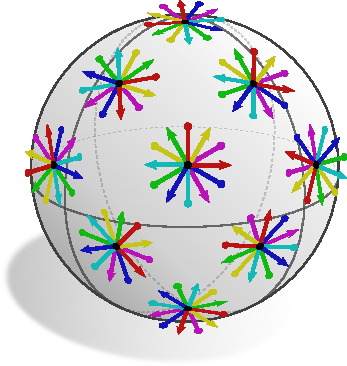
\includegraphics[width=.66\textwidth]{figures/G_structure_S2_1.pdf}
        \captionsetup{format=hang, width=.9\textwidth}
        \caption{\small
            $\SO2$-structure $\SOM$ on the 2-sphere $M=S^2$, preserved by general three-dimensional rotations in $\IsomSOM = \SO3$.
        }
        \label{fig:G_structure_S2_1}
    \end{subfigure}
    \hfill
    \begin{subfigure}[b]{0.48\textwidth}
        \centering
        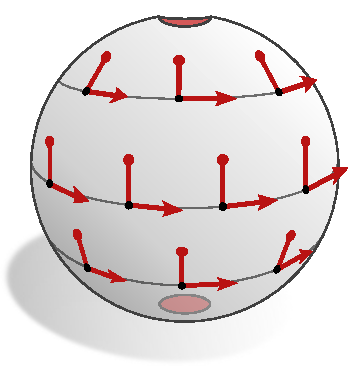
\includegraphics[width=.66\textwidth]{figures/G_structure_S2_2.pdf}
        \captionsetup{format=hang, width=.9\textwidth}
        \caption{\small
            $\{e\}$-structure $\eM$ on a punctured 2-sphere $M = S^2 \backslash \{n,s\}$, preserved by azimuthal rotations in $\IsomeM = \SO2$.
        }
        \label{fig:G_structure_S2_2}
    \end{subfigure}
    \vspace*{2ex}
    \caption{\small
        Common $G$-structures underlying spherical CNNs.
        Topological obstructions prevent a reduction of the 2-sphere's structure group beyond $G=\SO2$.
        Fig.~\ref{fig:G_structure_S2_1} shows the standard $\SO2$-structure on $S^2$, which is in agreement with the embedding metric (Eq.~\eqref{eq:spherical_embedding_metric_explicit}) induced from the inner product of $\R^3$.
        It is invariant under rotations in $\protect\IsomSOM = \SO3$, implying the rotation equivariance of the corresponding $\GM$-convolution.
        Note that the fibers $\GpM$ and $\GqM$ at different points $p$ and $q$ are isomorphic but not canonically so -- frame colors in the visualization seem to suggest such an isomorphism, however, they are randomly chosen and carry no meaning.
        %
        Fig.~\ref{fig:G_structure_S2_2} shows a sphere that is punctured at two antipodal poles.
        This turns the sphere into a topological cylinder $S^2 \backslash \{n,s\} \cong S^1\times(-\frac{\pi}{2},\frac{\pi}{2})$ with sphere like metric -- which allows for a complete reduction to a trivial structure group.
        The figure shows the most prominent choice of $\{e\}$-structure, which corresponds to orthonormal frames that are aligned with the coordinate grid of spherical coordinates; cf. Fig.~\ref{fig:spherical_equirectangular_1}.
        As this $\{e\}$-structure is invariant under azimuthal rotations around the polar axis, the corresponding $\GM$-convolutions are $\protect\IsomeM = \SO2$-equivariant.
        Note that the puncturing of the sphere is just a means of hiding the models' discontinuity at the poles.
    }
    \label{fig:G_structures_S2_main}
\end{figure}
